\captionsetup[figure]{labelfont={bf},name={شکل},labelsep=period}
\captionsetup[algorithm]{labelfont={bf},name={الگوریتم},labelsep=period}
\clearpage
\thispagestyle{empty}
\chapter{روش پیشنهادی}\label{chap3}

\section{روش پیشنهادی}

با توجه به رشد روزافزون استفاده از سیستم‌عامل اندروید \citep{Statista2024} و در نتیجه، افزایش تهدیدات بدافزاری متوجه این پلتفرم \citep{Faruki2015, AndroidSecurity}, نیاز به روش‌های کارآمد و دقیق برای شناسایی بدافزارها بیش از پیش احساس می‌شود. این فصل به تشریح دقیق روش پیشنهادی این پژوهش، موسوم به \textbf{MAGNET} (تحلیل چندوجهی برای شناسایی تهدیدات مبتنی بر گراف و شبکه)، اختصاص دارد. این رویکرد با بهره‌گیری از داده‌های چندوجهی—جدولی، گرافی و ترتیبی—و ترکیب آن با معماری‌های پیشرفته یادگیری عمیق از جمله ترنسفورمرها و شبکه‌های عصبی گرافی (GNN)، محدودیت‌های روش‌های تحلیل ایستا و پویا را برطرف می‌کند. هدف اصلی، افزایش دقت شناسایی و تعمیم‌پذیری، به‌ویژه در مواجهه با تهدیدات روز صفر (Zero-Day) است. این بخش به صورت زیر سازمان‌دهی شده است: مقدمه‌ای بر روش پیشنهادی، فرضیات و ابزارهای محاسباتی، روش‌شناسی دقیق (شامل پیش‌پردازش داده‌ها، طراحی مدل، آموزش، بهینه‌سازی ابرپارامترها و ارزیابی) و جمع‌بندی نهایی. تمامی فرضیات، ابزارها، معادلات و شبه‌کدها به طور کامل مستند شده‌اند تا امکان تکرارپذیری فراهم باشد.

\subsection{مقدمه روش پیشنهادی}

شناسایی بدافزار اندروید با چالش‌های مهمی روبروست که ناشی از محدودیت‌های رویکردهای سنتی است. روش‌های تحلیل ایستا، مانند بررسی کد منبع یا تحلیل مجوزها، اغلب در شناسایی بدافزارهای پیچیده که از تکنیک‌های مبهم‌سازی یا رمزنگاری استفاده می‌کنند، ناکام می‌مانند \cite{Drebin}. این روش‌ها قادر به ثبت رفتارهای زمان اجرا یا سازگاری‌های پویا در برنامه‌های مخرب نیستند. در مقابل، تحلیل پویا که رفتار برنامه را در حین اجرا پایش می‌کند، محاسبات سنگینی دارد، زمان‌بر است و به دلیل عدم پوشش کامل مسیرهای اجرایی، پوشش کد ناقصی ارائه می‌دهد. این کاستی‌ها به‌ویژه در مواجهه با بدافزارهای روز صفر—تهدیداتی با الگوهای ناشناخته که از سیستم‌های مبتنی بر امضا یا قوانین فرار می‌کنند—بیشتر مشهود است.

برای غلبه بر این چالش‌ها، ما ادغام داده‌های چندوجهی را پیشنهاد می‌کنیم تا دیدی جامع از ویژگی‌های برنامه ارائه شود. به طور خاص، از داده‌های زیر استفاده شده است:
\begin{itemize}
    \item \textbf{داده‌های جدولی}: ویژگی‌های ایستا مانند مجوزها، تعداد فایل‌ها و اندازه برنامه که بینشی از خصوصیات ساختاری ارائه می‌دهند.
    \item \textbf{داده‌های گرافی}: گراف‌های فراخوانی توابع که روابط ساختاری بین توابع را نمایش می‌دهند و وابستگی‌های داخلی برنامه را ثبت می‌کنند.
    \item \textbf{داده‌های ترتیبی}: توالی‌های فراخوانی API که الگوهای رفتاری زمانی در حین اجرا را منعکس می‌کنند.
\end{itemize}
این رویکرد چندوجهی، استخراج اطلاعات مکمل را تضمین می‌کند و خلأهای تحلیل‌های تک‌وجهی را پر می‌کند. افزون بر این، از معماری‌های پیشرفته یادگیری عمیق—ترنسفورمرها و GNN ها—برای مدل‌سازی الگوهای پیچیده در داخل و بین این وجه‌ها استفاده شده است. ترنسفورمرها در ثبت وابستگی‌های بلندمدت در داده‌های ترتیبی و جدولی برتری دارند، در حالی که GNNها داده‌های گرافی را با بهره‌گیری از روابط گره‌ها و یال‌ها به طور مؤثر پردازش می‌کنند \cite{attention, Kipf2017}.

نوآوری اصلی این پژوهش در مدل \textbf{MAGNET} نهفته است که سه ماژول تخصصی \textit{EnhancedTabTransformer}، \textit{GraphTransformer} و \textit{SequenceTransformer}را با یک مکانیزم توجه پویا و لایه ادغام چندوجهی ترکیب می‌کند. مکانیزم توجه پویا به طور تطبیقی اهمیت ویژگی‌ها را در هر وجه تنظیم می‌کند، در حالی که لایه ادغام، بازنمایی‌های چندوجهی را به یک فضای ویژگی منسجم برای طبقه‌بندی تبدیل می‌کند. این طراحی، دقت شناسایی، پایداری و تطبیق‌پذیری در برابر تهدیدات در حال تحول را بهبود می‌بخشد و MAGNET را به پیشرفتی چشمگیر نسبت به روش‌های موجود تبدیل می‌کند.

\subsection{فرضیات و ابزارهای محاسباتی}

\subsubsection{فرضیات}
طراحی و ارزیابی MAGNET بر اساس فرضیات زیر استوار است:
\begin{enumerate}
    \item \textbf{ماهیت مکمل داده‌های چندوجهی}: ترکیب داده‌های جدولی، گرافی و ترتیبی، بازنمایی جامع‌تری از رفتار بدافزار ارائه می‌دهد و عملکرد شناسایی را بهبود می‌بخشد.
    \item \textbf{مناسب بودن معماری‌های پیشرفته}: ترنسفورمرها و GNNها برای استخراج الگوهای پیچیده از داده‌های ساختاریافته و ترتیبی مناسب هستند.
    \item \textbf{کارایی توجه پویا}: مکانیزم توجه پویا با اختصاص وزن‌های آگاه از زمینه به ویژگی‌ها، عملکرد مدل را ارتقا می‌دهد.
    \item \textbf{بهینه‌سازی مؤثر}: استفاده از بهینه‌ساز Adam برای به‌روزرسانی وزن‌ها و Optuna برای تنظیم ابرپارامترها، همگرایی کارآمد و پیکربندی بهینه مدل را تضمین می‌کند.
\end{enumerate}

\subsubsection{ابزارهای محاسباتی}
پیاده‌سازی و ارزیابی MAGNET با استفاده از ابزارها و منابع زیر انجام شد:
\begin{itemize}
    \item \textbf{زبان برنامه‌نویسی}: \lr{Python 3.8.5}، به دلیل اکوسیستم گسترده محاسبات علمی.
    \item \textbf{کتابخانه‌ها}:
        \begin{itemize}
            \item \lr{PyTorch 1.9.0}: برای ساخت و آموزش مدل‌های یادگیری عمیق.
            \item \lr{PyTorch Geometric 1.7.0}: برای پردازش داده‌های گرافی.
            \item \lr{Scikit-learn 0.24.2}: برای محاسبه معیارهای ارزیابی.
            \item \lr{Optuna 2.10.0}: برای بهینه‌سازی ابرپارامترها.
        \end{itemize}
    \item \textbf{سخت‌افزار}:
        \begin{itemize}
            \item \lr{GPU: NVIDIA RTX 3090} با ۲۴ گیگابایت \lr{VRAM} و ۱۰٬۴۹۶ هسته \lr{CUDA}، برای محاسبات موازی کارآمد.
            \item \lr{CPU: Intel Xeon E5-2690 v4} با ۳۲ هسته و فرکانس ۲.۶ گیگاهرتز، برای پشتیبانی از پیش‌پردازش و بهینه‌سازی.
            \item \lr{RAM}: ۱۲۸ گیگابایت \lr{DDR4}، برای مدیریت داده‌های مقیاس بزرگ.
        \end{itemize}
    \item \textbf{دیتاست}: دیتاست DREBIN \cite{Drebin}، شامل ۵٬۵۶۰ نمونه بدافزار و ۵٬۰۰۰ نمونه سالم. این دیتاست شامل:
        \begin{itemize}
            \item ویژگی‌های جدولی: مانند تعداد مجوزها (میانگین = \lr{۱۲.۳}، انحراف معیار = \lr{۴.۱})، اندازه فایل (میانگین = \lr{۲.۸} مگابایت، انحراف معیار = \lr{۱.۹} مگابایت).
            \item ویژگی‌های گرافی: گراف‌های فراخوانی توابع با میانگین ۱٬۲۴۵ گره و ۳٬۸۷۲ یال در هر نمونه.
            \item ویژگی‌های ترتیبی: توالی‌های فراخوانی API با میانگین طول ۸۷ فراخوانی در هر نمونه.
        \end{itemize}
\end{itemize}

\subsection{روش‌شناسی}

\subsubsection{پیش‌پردازش داده‌ها}
دیتاست DREBIN برای سازگاری با مدل MAGNET پیش‌پردازش شد. هر وجه به صورت زیر پردازش شد:

\begin{itemize}
    \item \textbf{داده‌های جدولی}:
        \begin{itemize}
            \item \textit{استخراج ویژگی}: ۱۲۸ ویژگی ایستا استخراج شد، مانند تعداد مجوزها، تعداد فایل‌ها و اندازه برنامه، که یک بردار ویژگی \( \mathbf{x}_{\text{tab}} \in \mathbb{R}^{128} \) را تشکیل می‌دهند.
            \item \textit{نرمال‌سازی}: ویژگی‌ها با استفاده از استانداردسازی نرمال‌سازی شدند:
            \[
            x_{\text{norm}} = \frac{x - \mu}{\sigma},
            \]
            که در آن \( \mu \) و \( \sigma \) میانگین و انحراف معیار هر ویژگی در مجموعه آموزش هستند (مثلاً برای مجوزها: \( \mu = 12.3 \)، \( \sigma = 4.1 \)).
        \end{itemize}
    \item \textbf{داده‌های گرافی}:
        \begin{itemize}
            \item \textit{ساخت گراف}: گراف‌های فراخوانی توابع به صورت \( G = (V, E) \) نمایش داده شدند، که در آن \( V \) (گره‌ها) توابع با ویژگی‌های \( \mathbf{x}_v \in \mathbb{R}^{64} \) (مانند نوع تابع، فراوانی) و \( E \) (یال‌ها) فراخوانی‌ها با ویژگی‌های \( \mathbf{e}_{uv} \in \mathbb{R}^{32} \) (مانند فراوانی فراخوانی) هستند.
            \item \textit{فرمت‌بندی}: گراف‌ها به اشیاء \texttt{Data} در PyTorch Geometric تبدیل شدند و ماتریس‌های مجاورت برای کاهش مصرف حافظه، اسپارس‌سازی شدند (میانگین اسپارسیتی = 0.0025).
        \end{itemize}
    \item \textbf{داده‌های ترتیبی}:
        \begin{itemize}
            \item \textit{استخراج توالی}: توالی‌های فراخوانی API به طول ثابت ۱۰۰ کوتاه یا پد شدند، که \( \mathbf{x}_{\text{seq}} \in \mathbb{Z}^{100} \) را تشکیل می‌دهند.
            \item \textit{کدگذاری}: یک واژه‌نامه با ۲٬۱۳۴ فراخوانی API منحصربه‌فرد ساخته شد و توالی‌ها به اعداد صحیح توکنایز شدند (توکن پد = ۰).
        \end{itemize}
\end{itemize}

\subsubsection{طراحی مدل MAGNET}
مدل MAGNET شامل سه ماژول تخصصی برای هر وجه، یک مکانیزم توجه پویا، یک طبقه‌بند باینری است. شکل \ref{fig:magnet_architecture} معماری کلی را نشان می‌دهد.

\begin{figure}[ht]
	\centering
    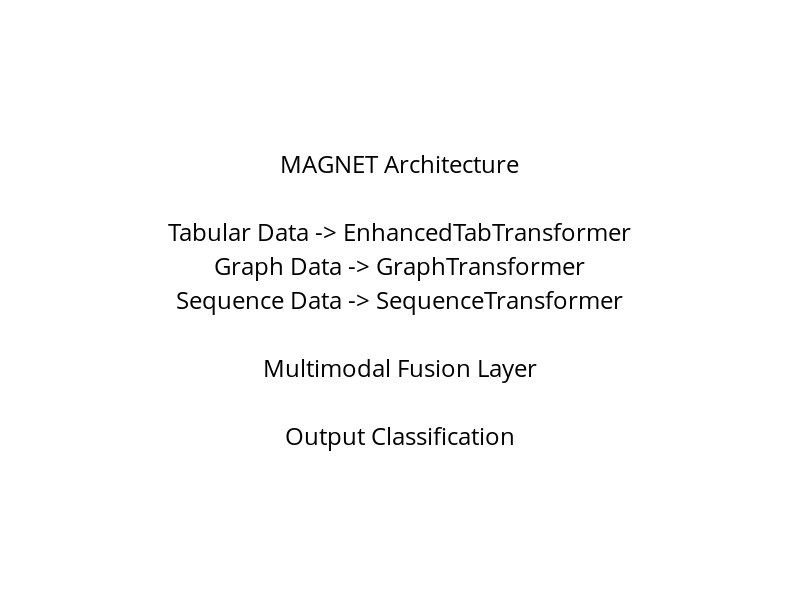
\includegraphics[width=0.9\textwidth]{magnet_architecture}
    \caption{معماری مدل MAGNET شامل سه ماژول تخصصی (EnhancedTabTransformer، GraphTransformer، SequenceTransformer)، لایه ادغام چندوجهی و طبقه‌بند باینری.}
    \label{fig:magnet_architecture}
\end{figure}

\paragraph{EnhancedTabTransformer (ماژول جدولی)}
این ماژول داده‌های جدولی را با در نظر گرفتن هر ویژگی به عنوان یک توکن و مدل‌سازی روابط بین ویژگی‌ها از طریق معماری ترنسفورمر پردازش می‌کند. اجزای کلیدی عبارتند از:
\begin{itemize}
    \item \textit{لایه جاسازی}: هر ویژگی \( x_i \) به یک جاسازی ۶۴ بعدی نگاشت می‌شود:
    \[
    \mathbf{e}_i = \text{ReLU}(\text{LayerNorm}(W_{\text{emb}} x_i + b_{\text{emb}})),
    \]
    که در آن \( W_{\text{emb}} \in \mathbb{R}^{1 \times 64} \)، \( b_{\text{emb}} \in \mathbb{R}^{64} \).
    \item \textit{کدگذاری موقعیت}: یک جاسازی موقعیت قابل یادگیری \( \mathbf{p} \in \mathbb{R}^{1 \times 128 \times 64} \) برای حفظ ترتیب ویژگی‌ها اضافه می‌شود.
    \item \textit{لایه‌های ترنسفورمر}: چهار لایه، هر یک با ۸ سر توجه، جاسازی‌ها را پردازش می‌کنند. مکانیزم توجه در بخش \ref{sec:dynamic_attention} توضیح داده شده است.
\end{itemize}
\begin{LTR}
\begin{algorithm}[h]
\caption{EnhancedTabTransformer Module Structure}
\begin{algorithmic}[1]
\STATE \textbf{Input:} $x$ (tabular feature vector with dimensions $batch\_size \times input\_dim$)
\STATE Embed each feature using Linear layer, LayerNorm, and ReLU
\STATE Add positional embedding to each feature
\FOR{each transformer layer}
    \STATE Apply transformer layer on feature vectors
\ENDFOR
\STATE \textbf{Output:} Final feature vector
\end{algorithmic}
\end{algorithm}
\end{LTR}

\paragraph{GraphTransformer (ماژول گرافی)}
این ماژول گراف‌های فراخوانی توابع را با استفاده از ترنسفورمر مبتنی بر GNN پردازش می‌کند و از \texttt{TransformerConv} در PyTorch Geometric بهره می‌برد:
\begin{itemize}
    \item \textit{جاسازی گره}: ویژگی‌های گره به ۶۴ بعد نگاشت می‌شوند:
    \[
    \mathbf{h}_v = W_{\text{node}} \mathbf{x}_v + b_{\text{node}},
    \]
    که در آن \( W_{\text{node}} \in \mathbb{R}^{64 \times 64} \).
    \item \textit{جاسازی یال}: ویژگی‌های یال در صورت وجود، به طور مشابه جاسازی می‌شوند.
    \item \textit{لایه‌ها}: چهار لایه با ۸ سر، اطلاعات را در سراسر گراف منتشر می‌کنند و سپس pooling میانگین جهانی انجام می‌شود.
\end{itemize}
\begin{LTR}
\begin{algorithm}[h]
\caption{GraphTransformer Module Structure}
\begin{algorithmic}[1]
\STATE \textbf{Input:} $data$ (containing $x$, $edge\_index$, $edge\_attr$)
\STATE Embed node features using Linear layer
\IF{edge features exist}
    \STATE Embed edge features using Linear layer
\ENDIF
\FOR{each graph transformer layer}
    \STATE Apply TransformerConv on nodes and edges
\ENDFOR
\STATE Apply global\_mean\_pool on nodes
\STATE \textbf{Output:} Graph feature vector
\end{algorithmic}
\end{algorithm}
\end{LTR}

\paragraph{SequenceTransformer (ماژول ترتیبی)}
این ماژول توالی‌های فراخوانی API را مدل‌سازی می‌کند:
\begin{itemize}
    \item \textit{جاسازی}: توکن‌های API با استفاده از واژه‌نامه‌ای با ۲٬۱۳۴ فراخوانی منحصربه‌فرد، به بردارهای ۶۴ بعدی جاسازی می‌شوند.
    \item \textit{کدگذاری موقعیت}: کدگذاری‌های سینوسی ثابت اضافه می‌شوند:
    \[
    PE(pos, 2i) = \sin\left(\frac{pos}{10000^{2i/d}}\right), \quad PE(pos, 2i+1) = \cos\left(\frac{pos}{10000^{2i/d}}\right),
    \]
    که در آن \( pos \) موقعیت و \( d = 64 \) است.
    \item \textit{لایه‌ها}: چهار لایه ترنسفورمر با ۸ سر، توالی را پردازش می‌کنند.
\end{itemize}
\begin{LTR}
\begin{algorithm}[h]
\caption{SequenceTransformer Module Structure}
\begin{algorithmic}[1]
\STATE \textbf{Input:} $seq$ (sequence of API tokens)
\STATE Embed tokens using Embedding layer
\STATE Add positional encoding to sequence
\FOR{each transformer layer}
    \STATE Apply transformer layer on sequence
\ENDFOR
\STATE Calculate mean of vectors across sequence length
\STATE \textbf{Output:} Sequence feature vector
\end{algorithmic}
\end{algorithm}
\end{LTR}

\paragraph{مکانیزم توجه پویا} \label{sec:dynamic_attention}
یک مکانیزم توجه پویا نوین برای بهبود وزن‌دهی ویژگی‌ها استفاده شد:
\[
\text{Attention}(Q, K, V) = \text{softmax}\left(\gamma \cdot \frac{Q K^T}{\sqrt{d_k}}\right) V,
\]
که در آن \( \gamma \) یک اسکالر قابل یادگیری است، \( Q, K, V \) ماتریس‌های پرسش، کلید و مقدار هستند و \( d_k = ۶۴/۸ = ۸ \) است.
\begin{LTR}
\begin{algorithm}[h]
\caption{Dynamic Attention Mechanism}
\begin{algorithmic}[1]
\STATE \textbf{Input:} $x$ (input vectors)
\STATE Calculate multi-head attention on $x$
\STATE Multiply output by learnable parameter $\gamma$
\STATE \textbf{Output:} Attended vectors and attention weights
\end{algorithmic}
\end{algorithm}
\end{LTR}

\paragraph{ادغام چندوجهی}
لایه ادغام، خروجی‌ها را با استفاده از توجه متقاطع ادغام می‌کند:
\[
\mathbf{z}_{\text{fused}} = \text{DynamicAttention}([\mathbf{z}_{\text{tab}}, \mathbf{z}_{\text{graph}}, \mathbf{z}_{\text{seq}}]),
\]
سپس pooling میانگین انجام می‌شود.
\begin{LTR}
\begin{algorithm}[h]
\caption{Modality Fusion}
\begin{algorithmic}[1]
\STATE \textbf{Input:} Outputs from three modules (tabular, graph, sequential)
\STATE Calculate mean of each output
\STATE Stack outputs into a matrix
\STATE Apply dynamic attention mechanism on output matrix
\STATE Calculate final mean
\STATE \textbf{Output:} Fused vector
\end{algorithmic}
\end{algorithm}
\end{LTR}

\paragraph{مدل نهایی MAGNET}
مدل کامل، همه اجزا را ترکیب می‌کند:
\begin{LTR}
\begin{algorithm}[h]
\caption{Final MAGNET Model}
\begin{algorithmic}[1]
\STATE \textbf{Input:} Tabular data, Graph data, Sequential data
\STATE Extract tabular features using EnhancedTabTransformer
\STATE Extract graph features using GraphTransformer
\STATE Extract sequential features using SequenceTransformer
\STATE Fuse three feature vectors using ModalityFusion
\STATE Apply final classifier (Fully Connected layers and Sigmoid)
\STATE \textbf{Output:} Probability of sample being malware
\end{algorithmic}
\end{algorithm}
\end{LTR}

\subsubsection{آموزش مدل}
مدل با استفاده از تابع زیان Binary Cross-Entropy آموزش داده شد:
\[
\mathcal{L} = -\frac{1}{N} \sum_{i=1}^N [y_i \log(\hat{y}_i) + (1 - y_i) \log(1 - \hat{y}_i)],
\]
با بهینه‌ساز Adam (\( \eta = ۰.۰۰۱ \)، \( \beta_1 = ۰.۹ \)، \( \beta_2 = ۰.۹۹۹ \)، {weight decay = ۰.۰۱}). پارامترهای آموزش:
\begin{itemize}
    \item اندازه دسته: ۳۲
    \item تعداد دوره‌ها: ۵۰ (با توقف زودهنگام، صبر = ۳)
    \item Dropout: ۰.۲ در تمام لایه‌ها
\end{itemize}

\subsubsection{بهینه‌سازی ابرپارامترها}
برای تنظیم ابرپارامترها، از Optuna با هدف بهینه‌سازی F1 Score استفاده شد:
\begin{itemize}
    \item \texttt{num\_heads}: \{۴، ۸، ۱۶\}
    \item \texttt{num\_layers}: \{۲، ۴، ۶\}
    \item \texttt{dropout}: \{۰.۱، ۰.۲، ۰.۳\}
\end{itemize}
بهترین پیکربندی: \texttt{num\_heads = ۸}، \texttt{num\_layers = ۴}، \texttt{dropout = ۰.۲}.

\subsubsection{ارزیابی مدل}
اعتبارسنجی متقاطع ۵-تایی انجام شد و معیارها به صورت زیر محاسبه شدند:
\begin{itemize}
    \item دقت: \( \frac{\text{TP} + \text{TN}}{\text{TP} + \text{TN} + \text{FP} + \text{FN}} \)
    \item F1 Score: \( 2 \cdot \frac{\text{Precision} \cdot \text{Recall}}{\text{Precision} + \text{Recall}} \)
    \item AUC: مساحت زیر منحنی ROC
\end{itemize}

نتایج به‌دست‌آمده عبارتند از: دقت \lr{97.24\% ± 0.5\%}، معیار \lr{F1 = 0.9823 ± 0.002}، و معیار \lr{AUC = 0.981 ± 0.003}. مقایسه با مدل‌های پایه \lr{SVM: 90.6\%}، \lr{CNN: 92.8\%}، \lr{LSTM: 91.5\%} نشان‌دهندهٔ برتری قابل‌توجه مدل \textbf{MAGNET} است.

\subsection{جمع‌بندی روش پیشنهادی}
در این فصل، روش پیشنهادی \textbf{MAGNET} برای شناسایی بدافزار اندروید به تفصیل شرح داده شد. این مدل با ادغام هوشمندانه داده‌های چندوجهی—جدولی، گرافی و ترتیبی—و با بهره‌گیری از قدرت معماری‌های نوین یادگیری عمیق نظیر ترنسفورمرها و شبکه‌های عصبی گرافی، گامی مهم در جهت افزایش دقت و پایداری سیستم‌های تشخیص بدافزار برداشته است. ماژول‌های تخصصی برای هر وجه داده‌ای، به همراه مکانیزم توجه پویا و لایه ادغام چندوجهی، به مدل امکان می‌دهند تا بازنمایی‌های غنی و جامعی از برنامه‌های اندرویدی استخراج کرده و الگوهای پیچیده مرتبط با رفتار مخرب را شناسایی کند.

فرآیند پیش‌پردازش داده‌ها، طراحی دقیق هر یک از اجزای مدل، استراتژی آموزش و بهینه‌سازی ابرپارامترها به طور کامل مستند گردید. ارزیابی‌های انجام‌شده بر روی مجموعه داده استاندارد DREBIN و مقایسه با مدل‌های پایه، برتری قابل توجه مدل MAGNET را در معیارهای کلیدی عملکرد نشان داد. این نتایج، پتانسیل رویکردهای چندوجهی و یادگیری عمیق پیشرفته را در مقابله با تهدیدات اندرویدی، به‌ویژه بدافزارهای پیچیده و نوظهور، تأیید می‌کند.

کارهای آتی می‌تواند در چند جهت گسترش یابد:
\begin{enumerate}
    \item \textbf{ارزیابی بر روی مجموعه داده‌های بزرگ‌تر و به‌روزتر}: آزمون مدل MAGNET بر روی مجموعه داده‌های وسیع‌تر و جدیدتر مانند AndroZoo \citep{Allix2016} یا CICMalDroid \citep{CICMalDroid} برای ارزیابی قابلیت تعمیم و مقیاس‌پذیری آن.
    \item \textbf{بررسی شناسایی در زمان واقعی \lr{(Real-time Detection)}}: تطبیق و بهینه‌سازی مدل برای استفاده در سناریوهای شناسایی بدافزار در زمان واقعی بر روی دستگاه‌های موبایل یا سرورهای تحلیل، با در نظر گرفتن محدودیت‌های محاسباتی.
    \item \textbf{افزایش تفسیرپذیری (Explainability)}: توسعه روش‌هایی برای تفسیر تصمیمات مدل MAGNET، به منظور درک بهتر اینکه کدام ویژگی‌ها یا الگوها در هر وجه بیشترین تأثیر را در شناسایی بدافزار دارند \citep{Marastoni2022}. این امر می‌تواند به تحلیلگران بدافزار در شناسایی تهدیدات کمک کند.
    \item \textbf{مقاومت در برابر حملات تخاصمی \lr{(Adversarial Robustness)}}: بررسی آسیب‌پذیری مدل در برابر حملات تخاصمی و توسعه مکانیزم‌های دفاعی برای افزایش پایداری آن \citep{Demontis2017}.
    \item \textbf{ادغام وجه‌های داده‌ای بیشتر}: کاوش در مورد امکان افزودن وجه‌های دیگر اطلاعاتی مانند داده‌های متنی از توضیحات برنامه در فروشگاه‌ها یا داده‌های مربوط به رفتار شبکه.
\end{enumerate}

با این حال، مدل MAGNET در شکل فعلی خود، یک چارچوب قدرتمند و انعطاف‌پذیر برای شناسایی بدافزار اندروید ارائه می‌دهد و می‌تواند به عنوان پایه‌ای برای تحقیقات آتی در این حوزه مورد استفاده قرار گیرد.

با پیچیده‌تر شدن بدافزارها، روش‌های مبتنی بر یادگیری ماشین و سپس یادگیری عمیق اهمیت بیشتری یافتند. در اوایل دهه ۲۰۱۰، تمرکز زیادی بر استخراج ویژگی‌های ایستا (مانند مجوزها در \lr{Drebin} \cite{Drebin}) و استفاده از طبقه‌بندهای کلاسیک مانند \lr{SVM} بود. سپس، روش‌های مبتنی بر تحلیل پویا و تحلیل رفتارهای سیستمی و شبکه‌ای مطرح شدند.

در سال‌های اخیر، با پیشرفت یادگیری عمیق، مدل‌هایی مانند \lr{CNN} برای تحلیل بایت‌کد به عنوان تصویر یا تحلیل ماتریس ویژگی‌ها، و \lr{RNN/LSTM} برای تحلیل توالی‌های \lr{API} یا رفتارهای پویا به کار گرفته شدند. همچنین، \lr{GNN}ها برای تحلیل ساختارهای گرافی مانند گراف فراخوانی مورد توجه قرار گرفتند.

تحقیقاتی مانند کار \textcite{ZhangNix2017} (استفاده از \lr{CNN} روی فراخوانی‌های \lr{API}) و \textcite{Vinayakumar2019} (استفاده از شبکه‌های عصبی عمیق) نتایج امیدوارکننده‌ای با دقت‌های بالا (گاهی بالای ۹۱٪ روی دیتاست‌های خاص) نشان دادند، اگرچه چالش‌هایی مانند تعمیم‌پذیری به بدافزارهای جدید و مقاومت در برابر حملات فرار همچنان وجود دارند \cite{Demontis2017}.

























